\documentclass[12pt]{article}

\usepackage[utf8]{inputenc}
\usepackage[a4paper, margin=1in]{geometry}
\usepackage{booktabs}
\usepackage{physics}
\usepackage{amsmath}
\usepackage{amsfonts}
\usepackage{graphicx}
\usepackage{siunitx}

\graphicspath{{./figures}}

\title{Physical Climatology (AES 630) Homework 3}
\author{Mitchell Dodson}
\date{September 25, 2023}

\newcommand*{\problem}[2]{
    \begin{table}[ht]
    \centering
        \begin{tabular}{ | p{.1\linewidth} p{.9\linewidth} | }
            \hline
            \vspace{.3em}\textbf{\large#1:} & \vspace{.3em}\small{#2}\hspace{.2em}\vspace{.5em} \\ \hline
        \end{tabular}
    \end{table}
}

\begin{document}

\maketitle


\problem{1.1}{
    Suppose a gas that absorbs insolation has uniform mass mixing ratio $M_a = 1\,\,\si{g.kg^{-1}}$, and absorption cross section $k_{abs} = 5\,\si{m^2.kg^{-1}}$.
    What altitude will the maximum rate of energy absorption per unit volume occur? Assume isothermal atmosphere temperature $T_a = 260\,\si{K}$,
    and surface pressure $P_s=\num{1.025e5}$ with a directly-overhead sun (solar zenith angle $\theta_0 = 0$ or $\mu_0 = \cos\left(\theta_0\right) = 1$).
}

\begin{equation}\label{tau_wrt_z}
    \tau = \frac{P_s}{g} M_a k_{abs} \exp\left[-\frac{z}{H}\right]
    = \frac{P_s}{g} M_a k_{abs} \exp\left[-\frac{zg}{RT_a}\right]
\end{equation}

%\begin{equation}
%\begin{split}
%    \frac{d\tau}{dz} &= -\frac{\tau}{H} = -\frac{\tau g}{RT} \\
%    & \rightarrow -\frac{RT_a}{g} \int \tau^{-1} d\tau = \int dz \\
%    & \rightarrow -\frac{287\,\si{J.kg^{-1}K^{-1}} \cdot 260\,\si{K}}{9.8 \,\si{m.s^{-2}}} \ln\left(\frac{\tau}{\ta}\right)
%\end{split}
%\end{equation}

Assuming a hydrostatic and isothermal atmosphere, the optical depth of an atmospheric constituent with a constant mass mixing ratio $M_a$ can be expressed
in terms of the hydrostatic balance with respect to sea level, as shown in Equation \ref{tau_wrt_z}.

\begin{equation}\label{q1_abs_rate}
    \frac{dF}{dz} = \frac{F_\infty}{H \mu_0} \cdot \tau \cdot \exp\left(-\frac{\tau}{\mu_0}\right)
\end{equation}

Under these atmospheric conditions, the volumetric absorption rate in $\,\si{W.m^{-3}}$ is modeled by Equation \ref{q1_abs_rate}.
Holding scale height as a constant due to the isothermal atmosphere...

\begin{equation}\label{q1_rate_wrt_tau}
\begin{split}
    0 &= \frac{d}{d\tau} \frac{dF}{dz} \\
    &= \frac{F_{\infty}}{\mu_0 H} \cdot\frac{d}{d\tau} \left(\tau \cdot \exp\left(-\frac{\tau}{\mu_0}\right)\right) \\
    &= \frac{F_{\infty}}{\mu_0 H} \cdot \exp\left(-\frac{\tau}{\mu_0}\right)\cdot\left(1-\frac{\tau}{\mu}\right) \\
\end{split}
\end{equation}

We can find the maximum absorption rate by solving for the zeros of Equation \ref{q1_abs_rate} with respect to absorption optical depth $\tau$,
as shown in Equation \ref{q1_rate_wrt_tau}. Since the first 2 terms in this equation must be greater than zero, there is only one valid solution at
$\tau = \mu_0$. Since $\mu_0 = 1$, the highest volumetric absorption occurs at total path optical depth $\tau = 1$.

\begin{equation}
\begin{split}
    H &:= -\frac{287\,\si{J.kg^{-1}.K^{-1}} \cdot 260\,\si{K}}{9.82\,\si{m.s^{-2}}} = 7,598.78 \,\si{m} \\
    a &:= \frac{9.82\,\si{m.s^{-2}}}{\num{1.025e5}\,\si{kg.m^{-1}.s^{-2}} \cdot 10^{-3} \,\si{kg.kg^{-1}} \cdot 5\,\si{m^2.kg^{-1}}} = \num{1.9161e-2} \\
    z &= -H \ln(a\tau)= -7,598.78\,\si{m} \cdot \ln(0.019161 \cdot 1) = 30,052.3\,\si{m} \\
\end{split}
\end{equation}

Thus the highest rate of absorption per unit volume is about $30.0523\,\si{km}$ above surface pressure given an isothermal and hydrostatically balanced atmosphere.

\problem{1.5}{
    Use the model of Fig 3.10, but distribute solar heating such that $0.3\,\sigma T_e^4$ is absorbed at each layer, and $0.4\,\sigma T_e^4$ is absorbed at the surface.
    Calculate the new equilibrium temperature profile. How does it differ from the case when all solar heating is applied at the surface?
}

\begin{equation}\label{lw_inv}
    \begin{split}
        \vec{S}
            &= A\vec{T} \implies  \vec{T} = A^{-1} \vec{S} \\
        \begin{pmatrix}-0.3\sigma \\ -0.3\sigma \\ -0.4\sigma\end{pmatrix}
            &= \begin{pmatrix} -2 & 1 & 0 \\ 1 & -2 & 1 \\ 0 & 1 & -1 \end{pmatrix}
                \begin{pmatrix} \sigma T_1^4 \\ \sigma T_2^4 \\ \sigma T_S^4 \end{pmatrix} \\
        \vec{T}^4
            &= \begin{pmatrix} -1 & -1 & -1 \\ -1 & -2 & -2 \\ -1 & -2 & -3 \end{pmatrix} \begin{pmatrix}-0.3 \\ -0.3 \\ -0.4\end{pmatrix} \\
        \begin{pmatrix} T_1 \\ T_2 \\ T_S \end{pmatrix}
            &= \begin{pmatrix} 1 \\ \sqrt[4]{1.7} \\ \sqrt[4]{2.1} \end{pmatrix} \approx \begin{pmatrix} 1 \\ 1.14186 \\ 1.2038 \end{pmatrix} \\
    \end{split}
\end{equation}

This problem considers a model with three layers that are opaque to longwave radiation, but share a ratio of shortwave flux absorption described by a vector $\vec{S}$,
consisting of the fraction of shortwave absorption in layers 1, 2, and the surface. Since the longwave absorption in each layer only depends on
the emission of adjacent layers, the longwave coefficients can be expressed as a linear symmetric matrix $A$.

The negative diagonal elements of $A$ correspond to each layer's number of emission directions (-2 for atmospheric layers, and -1 for the surface).
The off-diagonal unit elements represent the longwave emissions contributed to each layer by adjacent layers (proportionally to their temperature).

Given this model, the ratios between layer temperatures can be determined by inverting $A$ and using it to transform the shortwave abosption coefficients $S$
into the temperature ratios $T$, and cancelling out $\sigma$, as shown in Equation \ref{lw_inv}.

\begin{equation}\label{lw_dist_profile}
        \begin{pmatrix} T_1^4 \\ T_2^4 \\ T_S^4 \end{pmatrix}
            = \begin{pmatrix} T_e \\ T_e \sqrt[4]{1.7} \\ T_e \sqrt[4]{2.1} \end{pmatrix}
            = \begin{pmatrix} 255\,\si{K} \\ 291.17\,\si{K} \\ 306.97\,\si{K} \end{pmatrix}
\end{equation}

Since each layer acts as a blackbody in the longwave spectrum, the uppermost layer's temperature is the longwave emission temperature of earth at TOA.
Thus with $T_e = T_1$, and assuming the same planetary longwave brightness temperature as the textbook example $T_e = 255\si{K}$,
we find the equilibrium atmospheric profile in Equation \ref{lw_dist_profile}, and displayed in Figure \ref{3ly_compare}.

\begin{figure}[h!]
    \centering
    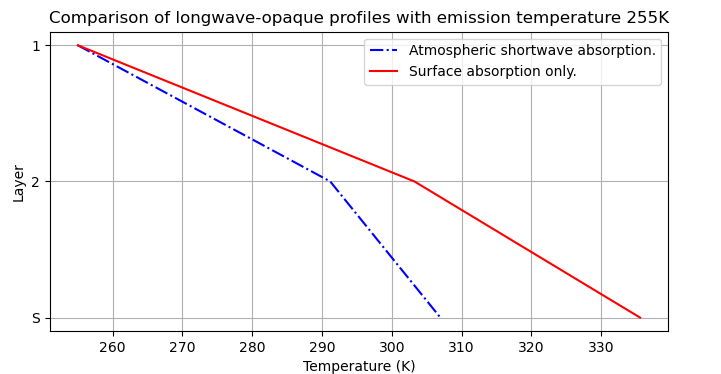
\includegraphics[width=.9\textwidth]{3-layer-temperature-comparison.png}
    \caption{Equilibrium temperature of a longwave-opaque 3-layer model with shortwave absorption distributed between layers compared to a similarly longwave-opaque 3-layer model with absorption only at the surface layer. }
    \label{3ly_compare}
\end{figure}


\begin{equation}\label{lw_sfc_profile}
    \begin{split}
        \begin{pmatrix} T_1^4 \\ T_2^4 \\ T_S^4 \end{pmatrix}
        &= \begin{pmatrix} -1 & -1 & -1 \\ -1 & -2 & -2 \\ -1 & -2 & -3 \end{pmatrix} \begin{pmatrix} 0 \\ 0 \\ -1 \end{pmatrix} \\
        \begin{pmatrix} T_1 \\ T_2 \\ T_S \end{pmatrix}
        &= \begin{pmatrix} T_e \\ T_e\sqrt[4]{2} \\ T_e\sqrt[4]{3}\end{pmatrix}
            = \begin{pmatrix} 255\,\si{K} \\ 303.25\,\si{K} \\ 335.6\,\si{K} \end{pmatrix} \\
    \end{split}
\end{equation}

The longwave absorption coefficient matrix $A$ is the same for the surface-only absorption model, but the absorption vector $S := [0,0,-1]$
since all shortwave radiation is contributed to the surface. As Equation \ref{lw_sfc_profile} and Figure \ref{3ly_compare} show, given radiative balance
and 3 atmospheric layers that are infrared blackbodies, the surface temperature is about $28.6\,\si{K}$ cooler in the model with atmospheric SW absorption,
and the layer 2 temperature is about $12.1\,\si{K}$ cooler in the model with atmospheric SW absorption.

\problem{1.6}{
    Place the two layers in the model of Fig. 3.10 at 2.5 and $5.0\,\si{km}$. With a fixed lapse rate $\Gamma = -6.5\,\si{K.km^{-1}}$,
    derive energy balance equations including an unknown convective energy flux from the surface to the lowest layer, and from the lowest layer to the upper layer.
    Solve for the temperature profile in thermal equilibrium, and find the required convective energy fluxes from the surface and the lower layer.
    How do radiative and convective fluxes compare with the proportions given in Figure 2.4?
}

\noindent
Let $t_i := \sigma T_i^4$ in $\si{W.m^{-2}}$, upper-level convective flux be $F_U$, and lower-level convective flux be $F_L$.

\begin{equation}
    \begin{split}\label{p6_balance}
        2t_1 &= t_2 + F_U \\
        2t_2 &= t_1 + t_s - F_U + F_L \\
        t_s &= t_e + t_2 - F_L \\
    \end{split}
\end{equation}

The energy balance for each layer including the convective transfer terms is expressed as in Equation \ref{p6_balance}.
Since the radiative model in Fig. 10 of (Hartman, 2016) has an equilibrium planetary emission temperature of $255\,\si{K}$,
I will assume the same for this model.

\begin{equation}\label{p6_temps}
    \begin{split}
        T_1 &= 255 \,\si{K} \\
        T_2 &= T_1 + (-2.5\,\si{km})\Gamma =  271.25 \,\si{K} \\
        T_S &= T_1 + (-5\,\si{km})\Gamma = 287.5 \,\si{K} \\
    \end{split}
\end{equation}

With a constant lapse rate of $\Gamma = -6.5\,\si{K.km^{-1}}$, the adjusted temperatures at each layer are calculated in Equation \ref{p6_temps}
by multiplying the lapse rate by each layer's elevation relative to the topmost layer 1.

\begin{equation}\label{p6_fluxes}
    \begin{split}
        F_U &= 2\,t_1 - t_2 = \sigma(2\,T_1^4-T_2^4) = 172.454\,\si{W.m^{-2}} \\
        F_L &= t_e + t_2 - t_s = \sigma(T_e^4 + T_2^4 -T_s^4) = 159.31\,\si{W.m^{-2}} \\
    \end{split}
\end{equation}

Solving for the upper and lower fluxes in Equation \ref{p6_fluxes}, we find that the lower layer contributes $172.454\,\si{W.m^{-2}}$ in convective flux to the upper layer,
and the surface provides $159.31\,\si{W.m^{-2}}$  to the lower layer. The amount of heat adjusted from lower to upper layers by convection in this model is considerably
higher than the convective and latent heat fluxes in (Hartman, 2016) Figure 2.4, which only total around $108\,\si{W.m^{-2}}$. This reflects the extremely high surface
temperature returned by the model in radiative equilibrium, which requires a large adjustment to maintain a realistic lapse rate.

\clearpage

\problem{1.8}{
    Suppose tropical convective clouds giving an average planetary albedo (with clouds) of $\alpha_c = 0.6$, compared to cloud-free albedo $\alpha_n = 0.1$.
    With insolation $S = 400\,\si{W.m^{-2}}$, cloud-free outgoing longwave radiation $F_n^\uparrow \approx 280\,\si{W.m^{-2}}$,
    use the simplified Sect. 3.11 model to find the cloud top temperature such that the net radiative effect of clouds is zero.
    Are the cloud top temperatures observed in the tropical troposphere, and if so where?
    If the surface temperature is $T_s = 300\,\si{K}$ with mean lapse rate $\Gamma = 5\,\si{K.km^{-1}}$, at what altitude would the cloud top be in order for the
    longwave and shortwave effects of the cloud to be equal and opposite?
}

\begin{equation}\label{q8_rads}
    \begin{split}
        R_{TOA} &= S(1-\alpha_p) - F_{\infty}^\uparrow \\
        R_c &= S (1-\alpha_c) - F_c^\uparrow \\
        &= 400\,\si{W.m^{-2}} \cdot (1-0.6) - F_c^\uparrow \\
        &=160\,\si{W.m^{-2}} - F_c^\uparrow \\
        R_n &= S (1-\alpha_n) - F_n^\uparrow \\
        &= 400\,\si{W.m^{-2}} \cdot (1-0.1) - 280\,\si{W.m^{-2}} \\
        &=80\,\si{W.m^{-2}} \\
    \end{split}
\end{equation}

In Equation \ref{q8_rads}, $R_c$ represents the TOA energy balance when there are clouds, and $R_n$ is the energy balance with no clouds.
Since $F_n$ is provided, we can solve for $R_n = 80\,\si{W.m^{-2}}$ directly, and find that the cloudy-sky radiative forcing $F_c^\uparrow = 160\,\si{W.m^{-2}}-R_c$.

\begin{equation}\label{q8_balance}
    \Delta R_{TOA} = R_c - R_n = 0 \implies R_n = R_c \implies F_c^\uparrow = 160-80 = 80\,\si{W.m^{-2}}
\end{equation}

\begin{equation}\label{q8_temp}
    T_c = \sqrt[4]{F_c^\uparrow \cdot \sigma^{-1}} = 193.81\,\si{K}
\end{equation}

With an energy balance $\Delta R_{TOA} = 0$,  cloudy-sky radiative forcing is $F_c^\uparrow = 80\,\si{W.m^{-2}}$, as shown in Equation \ref{q8_balance}.
Equation \ref{q8_temp} inverts the Stefan-Boltzmann equation to provide the cloudy-layer brightness temperature given the energy balance, $T_c = 193.81\,\si{K}$.
Figure 1.3 from the text suggests that temperatures like this around $-80^\circ C$ are only found near the tropical tropopause, near 17 or 18 $\si{km}$ above ground level.

\begin{equation}
    F_c^\uparrow = \frac{1}{2} S(1-\alpha_c) = 200\,\si{W.m^{-1}}\cdot(1-0.6) = 80\,\si{W.m^{-2}}
\end{equation}
\begin{equation}
    \begin{split}
        z_c &= \frac{1}{\Gamma}\left(\sqrt[4]{F_c^\uparrow}-T_{sfc}\right) = -\frac{1}{5}\left(\sqrt[4]{80\cdot\sigma^{-1}}-300\,\si{K}\right) \\
        &= 21.238\,\si{km}
    \end{split}
\end{equation}


If the shortwave and longwave components of the cloud's radiative forcing are equal and opposite, then $R_c = 0$ and $F_c^\uparrow = 80\,\si{W.m^{-2}}$.
Then, the difference between the cloud-top brightness temperature and provided surface temperature can be divided by the lapse rate $\Gamma = -5\,\si{K}{km}$
to estimate the cloud-top altitude $z_c = 21.238\,\si{km}$

\end{document}
